\section{Kết quả và thảo luận}
\label{sec:results}

Mọi số liệu trong mục này được sinh tự động từ \texttt{results/} bằng
\texttt{scripts/make\_figures.py}; mỗi câu hỏi có một dòng trong các tệp \texttt{.jsonl} đã commit.
Trừ khi ghi chú khác, $n=500$ câu hỏi, các vị trí đoạn vàng 1/10/20, reader Qwen2.5-7B-Instruct-AWQ.

%------------------------------------------------------------------------------
\subsection{Bộ nén giữ được bao nhiêu bằng chứng?}
\label{sec:res-recall}

Bảng~\ref{tab:recall} đo \emph{context recall} -- tỉ lệ câu hỏi mà đáp án còn nằm trong ngữ cảnh sau
nén -- cho mọi bộ nén mà không cần gọi LLM. Đây là trần trên của độ chính xác sau nén: nếu đáp án đã bị
xoá thì reader chỉ còn trả lời được bằng tri thức tham số (closed-book).

\begin{table}[t]
\centering
\caption{Context recall (\%) theo vị trí đoạn vàng, số token sau nén, tỉ lệ nén và độ trễ nén trung
bình mỗi câu hỏi (GPU). Bộ nén mức tài liệu/token/câu xử lý từng đoạn độc lập nên recall không phụ
thuộc vị trí. LongLLMLingua: $n=200$, chỉ vị trí 10.}
\label{tab:recall}
\small
\begin{tabular}{l r r r r r r}
\toprule
Bộ nén & Token & Nén & R@1 & R@10 & R@20 & ms/câu \\
\midrule
\inputtable{tables/recall.tex}
\bottomrule
\end{tabular}
\end{table}

\paragraph{Nhận xét.}
\begin{itemize}
  \item \textbf{Ở cùng mức nén $\approx$4$\times$, nén mức câu giữ bằng chứng tốt nhất}: Provence
  ($\tau=0{,}1$) giữ 91,6\% đáp án với 621 token (4,6$\times$), hơn Rerank top-5 (79,4\%) 12,2 điểm,
  hơn LongLLMLingua (77,5\%) và LLMLingua-2 $r=0{,}25$ (68,0\%) lần lượt 14 và 24 điểm. Cắt tỉa theo
  \emph{câu}, có điều kiện câu hỏi, giữ nguyên các câu chứa đáp án; còn bỏ token rời rạc (LLMLingua-2
  không nhìn câu hỏi) có thể làm mất chính thực thể cần trả lời.
  \item \textbf{Ở $\approx$2$\times$}, OpenProvence (96,4\%, 2,6$\times$) và Provence $\tau=0{,}01$
  (95,8\%, 2,5$\times$) gần như không mất bằng chứng; Rerank top-10 (89,8\%) và LLMLingua-2 $r=0{,}5$
  (88,2\%) mất khoảng 10\%.
  \item \textbf{BM25 kém trong bối cảnh này} (53,2\% ở top-5): 19 đoạn nhiễu của bộ dữ liệu vốn được
  Contriever truy hồi là ``hard negative'' có độ trùng từ vựng cao với câu hỏi. Cross-encoder MiniLM
  (22M tham số), đọc câu hỏi và đoạn cùng lúc, cho recall cao hơn bi-encoder bge-small 10,4 điểm mà
  vẫn nhanh hơn (14 so với 121 ms mỗi câu trong cài đặt của chúng tôi).
  \item \textbf{Truncate} đúng như kỳ vọng: giữ trọn đáp án khi đoạn vàng ở đầu và mất gần hết khi đoạn
  vàng ở giữa/cuối -- một baseline cho thấy vì sao cần nén \emph{có điều kiện câu hỏi}.
\end{itemize}

%------------------------------------------------------------------------------
\subsection{Độ chính xác của RAG sau nén}
\label{sec:res-main}

\begin{table}[t]
\centering
\caption{Kết quả chính (Qwen2.5-7B-Instruct-AWQ, $n=500$): accuracy (\%) theo vị trí đoạn vàng và
trung bình (TB), số token ngữ cảnh, tỉ lệ nén, context recall (\%) và độ trễ nén (ms/câu, GPU). BM25 và
Dense top-5 chỉ chạy ở vị trí 10 (đã có số công bố, Mục~\ref{sec:res-published}); LongLLMLingua
($n=200$) ở Bảng~\ref{tab:published}. In đậm: TB cao nhất trong các bộ nén.}
\label{tab:main}
\small
\setlength{\tabcolsep}{4pt}
\begin{tabular}{l r r r r r r r r}
\toprule
Cấu hình & @1 & @10 & @20 & TB & Token & Nén & Recall & ms \\
\midrule
\inputtable{tables/main_results.tex}
\end{tabular}
\end{table}

\begin{figure}[t]
\centering
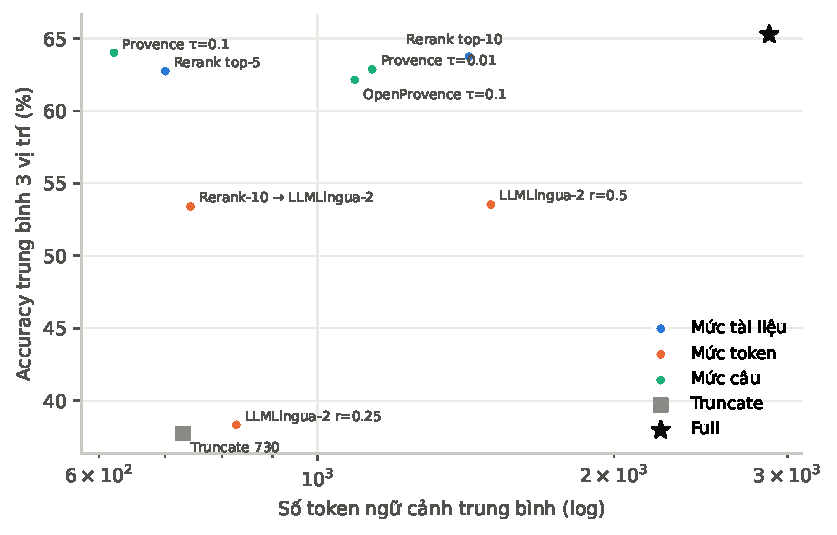
\includegraphics[width=0.8\linewidth]{tradeoff.pdf}
\caption{Accuracy trung bình 3 vị trí theo số token ngữ cảnh (thang log). Góc trên bên trái là tốt
nhất: ít token, độ chính xác cao.}
\label{fig:tradeoff}
\end{figure}

Bảng~\ref{tab:main} và Hình~\ref{fig:tradeoff} cho thấy khoảng cách giữa closed-book (38,8\%) và
oracle (92,6\%) là 53,8 điểm: ngữ cảnh rất quan trọng, nhưng 20 đoạn đầy đủ (65,3\%) chỉ khai thác được
một nửa khoảng cách đó vì nhiễu. Kiểm định bootstrap ghép cặp (10.000 lần lấy mẫu, khoảng tin cậy 95\%,
\texttt{results/compression/significance.csv}) so với ngữ cảnh đầy đủ cho các kết luận sau.

\begin{itemize}
  \item \textbf{Ở 4$\times$, nén mức câu gần như không mất độ chính xác.} Provence $\tau=0{,}1$ dùng
  621 token (4,6$\times$) và đạt 64,0\% so với 65,3\%; chênh lệch ở cả ba vị trí đều không có ý nghĩa
  thống kê ($-1{,}8$ [$-5{,}6$; $2{,}0$], $+0{,}4$ [$-3{,}4$; $4{,}2$], $-2{,}4$ [$-6{,}2$; $1{,}4$]
  điểm ở vị trí 1/10/20). Đây là cấu hình tốt nhất trên toàn bộ đường Pareto.
  \item \textbf{Chọn tài liệu bằng cross-encoder đứng thứ hai.} Rerank top-5 (4,1$\times$) đạt 62,7\%,
  nhưng giảm có ý nghĩa ở vị trí 20 ($-6{,}0$ [$-10{,}0$; $-2{,}2$]) vì 20,6\% câu mất đoạn chứa đáp án.
  Rerank top-10 (2$\times$) đạt 63,7\%. Bộ chọn rẻ hơn kém xa: Dense top-5 56,0\%, BM25 top-5 45,4\%
  (vị trí 10).
  \item \textbf{Nén mức token thất bại với reader 7B.} LLMLingua-2 $r=0{,}25$ (3,5$\times$) chỉ đạt
  38,3\% -- ngang closed-book -- dù context recall vẫn còn 68\%; ở $r=0{,}5$ (1,9$\times$) cũng chỉ
  53,5\%. Ghép rerank-10 trước LLMLingua-2 (cấu hình tốt nhất của LLMLingua-2 trên GPT-3.5) đạt 53,4\%,
  giảm có ý nghĩa ở mọi vị trí. Mục~\ref{sec:res-errors} cho thấy phần lớn thiệt hại không đến từ việc
  xoá đáp án mà từ việc văn bản bị xé vụn khiến reader đọc sai.
  \item \textbf{OpenProvence} (2,6$\times$) giữ bằng chứng tốt nhất (recall 96,4\%) nhưng accuracy
  62,1\%, thấp hơn Provence $\tau=0{,}1$ dù giữ nhiều token hơn: giữ thêm câu nhiễu không giúp reader.
  \item \textbf{Truncate} là trường hợp đặc biệt: khi đoạn vàng ở đầu, cắt còn 730 token lại
  \emph{tăng} accuracy lên 74,0\% ($+8{,}4$ [$5{,}0$; $12{,}0$]) vì loại bỏ 15 đoạn nhiễu; nhưng ở vị trí
  10/20 chỉ còn 19,6\%. Điều này xác nhận rằng ngữ cảnh ngắn và đúng tốt hơn ngữ cảnh dài -- vấn đề là
  chọn \emph{đúng} phần nào.
\end{itemize}

\paragraph{Chi phí.} Với vLLM, thời gian prefill tỉ lệ với số token: Provence giảm 2.875 $\to$ 621 token
mỗi câu, đổi lại khoảng 200 ms nén trên GPU (4,9 s trên CPU, Bảng~\ref{tab:latency}). Rerank top-5
rẻ hơn hẳn (16 ms GPU, 196 ms CPU) với độ chính xác thấp hơn 1,3 điểm -- là lựa chọn hợp lý khi không có
GPU.

%------------------------------------------------------------------------------
\subsection{Nén và hiện tượng \emph{lost in the middle}}
\label{sec:res-position}

\begin{figure}[t]
\centering
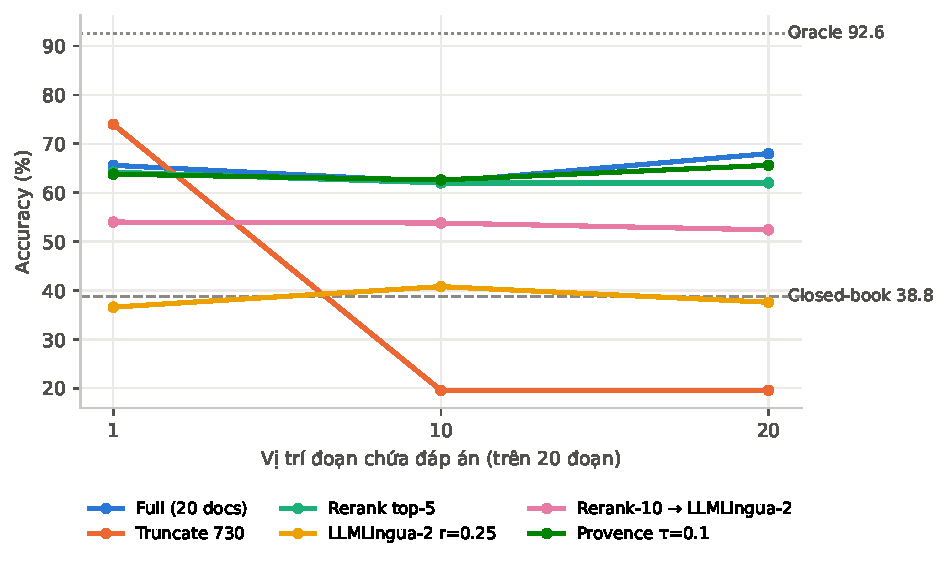
\includegraphics[width=0.8\linewidth]{position_curve.pdf}
\caption{Accuracy theo vị trí đoạn chứa đáp án. Đường ngang: closed-book và oracle.}
\label{fig:position}
\end{figure}

Với GPT-3.5-Turbo, \citet{liu2024lost} và LongLLMLingua báo cáo đường cong chữ U sâu: 75,7 / 54,1 /
63,1\% ở vị trí 1/10/20, chênh 21,6 điểm giữa đầu và giữa. Với Qwen2.5-7B-Instruct, đường cong của ngữ
cảnh đầy đủ gần như phẳng (65,6 / 62,2 / 68,0\%): chênh lệch lớn nhất chỉ 5,8 điểm, và vị trí cuối còn
tốt hơn vị trí đầu (Hình~\ref{fig:position}). Các mô hình mới được huấn luyện với ngữ cảnh dài hơn
nhiều (Qwen2.5: 32K--128K token) nên 2.900 token không còn là ngữ cảnh ``dài''.

Hệ quả là nén \emph{không có nhiều chỗ để làm phẳng} đường cong: Provence $\tau=0{,}1$ cho 63,8 / 62,6 /
65,6\%, gần như song song với ngữ cảnh đầy đủ. Các bộ nén không phụ thuộc vị trí (mức tài liệu, câu,
token) giữ nguyên hình dạng đường cong của reader; chỉ truncate -- vốn phụ thuộc vị trí -- tạo ra độ
dốc lớn.

%------------------------------------------------------------------------------
\subsection{Đối chiếu với số liệu đã công bố}
\label{sec:res-published}

\begin{table}[t]
\centering
\caption{So sánh với số liệu đã công bố trên cùng benchmark (GPT-3.5-Turbo-0613; LongLLMLingua
\citep{jiang2024longllmlingua} Bảng 1 và LLMLingua-2 \citep{pan2024llmlingua2} Bảng 4). Hàng đầu:
accuracy tuyệt đối (\%) của ngữ cảnh đầy đủ; các hàng sau: \emph{chênh lệch} (điểm) so với ngữ cảnh
đầy đủ của chính hệ đó. LongLLMLingua của chúng tôi: so cặp trên 193 câu chung với lần chạy đầy đủ.}
\label{tab:published}
\small
\setlength{\tabcolsep}{3.5pt}
\begin{tabular}{l r r r l r r r}
\toprule
\multicolumn{4}{c}{GPT-3.5-Turbo (đã công bố)} & \multicolumn{4}{c}{Qwen2.5-7B-AWQ (của chúng tôi)} \\
\cmidrule(lr){1-4}\cmidrule(lr){5-8}
Phương pháp & @1 & @10 & @20 & Cấu hình tương ứng & @1 & @10 & @20 \\
\midrule
\inputtable{tables/published.tex}
\bottomrule
\end{tabular}
\end{table}

Vì GPT-3.5-Turbo-0613 đã ngừng hoạt động, chúng tôi so sánh \emph{độ chênh so với baseline của chính
mỗi hệ} (Bảng~\ref{tab:published}) thay vì số tuyệt đối.
\begin{itemize}
  \item \textbf{Tái lập được}: thứ hạng giữa các bộ chọn tài liệu (SBERT/Dense tốt hơn BM25 rõ rệt) và
  mức sụt nặng của LLMLingua-2 đơn lẻ ở 4$\times$ ($-29{,}0$ / $-21{,}4$ / $-30{,}4$ điểm so với
  $-27{,}1$ / $-10{,}5$ / $-23{,}2$ được công bố).
  \item \textbf{Không tái lập được}: kết luận ``nén làm \emph{tăng} độ chính xác ở giữa'' -- LongLLMLingua
  $+17{,}1$ và LLMLingua-2 + lọc tài liệu $+12{,}9$ điểm ở vị trí 10. Với reader của chúng tôi, mức thay
  đổi tương ứng là $+1{,}0$ (không có ý nghĩa thống kê, khoảng tin cậy [$-6{,}7$; $8{,}8$]) và $-8{,}4$.
  Lời giải thích hợp lý nhất là ở Mục~\ref{sec:res-position}: lợi ích chính của các phương pháp này trên
  GPT-3.5 là \emph{khắc phục lost in the middle}, mà reader hiện đại hầu như không còn mắc.
  \item Về vị trí đầu và cuối, cả hai hệ đều cho thấy nén 4$\times$ ở mức tốt nhất chỉ \emph{hoà}
  với ngữ cảnh đầy đủ (LongLLMLingua $-0{,}7$ trên GPT-3.5; Provence $-1{,}8$ / $-2{,}4$ của chúng tôi).
\end{itemize}

%------------------------------------------------------------------------------
\subsection{Nén mềm}
\label{sec:res-soft}

\begin{table}[t]
\centering
\caption{Nén mềm so với văn bản trên \emph{cùng} một reader (accuracy \%, 500 câu/vị trí; rerank: chỉ
vị trí 10). Token: số vector nhớ hoặc token văn bản đưa vào reader; Nén: so với 20 đoạn văn bản.}
\label{tab:soft}
\small
\begin{tabular}{l r r r r r r}
\toprule
Cấu hình & @1 & @10 & @20 & TB & Token & Nén \\
\midrule
\inputtable{tables/soft.tex}
\end{tabular}
\end{table}

% TODO(T09): text for PISCO (T12) + own encode-once model (T16-T18)

%------------------------------------------------------------------------------
\subsection{Truy hồi hiệu quả}
\label{sec:res-retrieval}

Bảng~\ref{tab:retrieval} so sánh các retriever trên kho gộp 50,7k đoạn (mọi đoạn của 2.655 câu hỏi),
với 500 câu hỏi của tập đánh giá.

\begin{table}[t]
\centering
\caption{Truy hồi trên kho 50,7k đoạn ($n=500$). Hit@$k$: top-$k$ chứa đoạn có đáp án (\%); MRR@10
của đoạn vàng (\%); kích thước chỉ mục (MB); thời gian truy vấn mỗi câu khi chạy theo batch và khi
chạy từng câu (ms, GPU cho mô hình nhúng).}
\label{tab:retrieval}
\small
\begin{tabular}{l r r r r r r r}
\toprule
Hệ thống & Hit@1 & Hit@5 & Hit@20 & MRR@10 & MB & ms (batch) & ms (1 câu) \\
\midrule
\inputtable{tables/retrieval.tex}
\bottomrule
\end{tabular}
\end{table}

\begin{figure}[t]
\centering
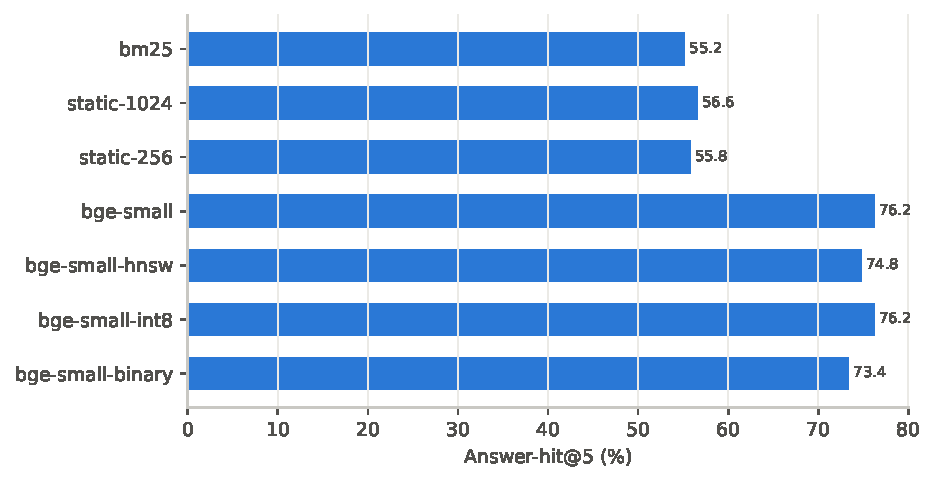
\includegraphics[width=0.75\linewidth]{retrieval_hit5.pdf}
\caption{Answer-hit@5 của các retriever trên kho 50,7k đoạn.}
\label{fig:retrieval}
\end{figure}

\paragraph{Nhận xét.}
\begin{itemize}
  \item \textbf{Retriever dày đặc nhỏ vượt xa BM25}: bge-small (33M) đạt hit@5 76,2\% so với 55,2\%
  của BM25S, MRR@10 53,8 so với 31,6.
  \item \textbf{Lượng tử int8 miễn phí}: chỉ mục giảm 4$\times$ (74,3 $\to$ 18,6 MB) mà hit@5 giữ
  nguyên 76,2\%; MRR@10 chỉ giảm 0,1 điểm.
  \item \textbf{Nhị phân + rescore}: chỉ mục 2,3 MB (32$\times$ nhỏ hơn) vẫn đạt 73,4\% hit@5 (mất 2,8
  điểm), hit@20 gần như không đổi (94,4 so với 95,4) -- phù hợp làm tầng truy hồi đầu, sau đó rerank.
  \item \textbf{Static embedding} (không có Transformer) ngang BM25 về chất lượng (55,8--56,6\%) và
  không cần GPU; cắt Matryoshka 1024 $\to$ 256 chiều giảm chỉ mục 4$\times$ chỉ mất 0,8 điểm hit@5.
  \item HNSW giảm độ trễ truy vấn đơn (12,6 $\to$ 5,5 ms) đổi lấy 1,4 điểm hit@5; ở quy mô 50k đoạn,
  tìm kiếm chính xác vẫn đủ nhanh.
\end{itemize}

%------------------------------------------------------------------------------
\subsection{Chạy không cần GPU}
\label{sec:res-cpu}

\begin{table}[t]
\centering
\caption{Độ trễ nén (trung vị ms/câu, 20 câu ở vị trí 10, gọi từng câu một sau 1 lần khởi động; không
tính LLM). GPU: RTX 4070 SUPER 12 GB; CPU: Core i5-14600K, 8 luồng.}
\label{tab:latency}
\small
\begin{tabular}{l r r r}
\toprule
Bộ nén & GPU (ms) & CPU (ms) & CPU/GPU \\
\midrule
\inputtable{tables/latency.tex}
\bottomrule
\end{tabular}
\end{table}

Câu hỏi thực tế của nhóm là: nếu không có GPU, phần nào của pipeline còn dùng được? Reader được gọi
qua API tương thích OpenAI (vLLM cục bộ hoặc dịch vụ trả phí), nên phần chạy cục bộ chỉ còn bộ nén.
Bảng~\ref{tab:latency} cho thấy ba nhóm rõ rệt:
\begin{itemize}
  \item \textbf{Mức tài liệu} (BM25, dense, rerank) chạy dưới 0,4 s/câu trên CPU -- đủ cho ứng dụng
  tương tác. Rerank top-5 (196 ms) giữ 62,7\% accuracy trung bình so với 65,3\% của ngữ cảnh đầy đủ ở
  4,1$\times$.
  \item \textbf{Mức câu} (OpenProvence, Provence) chậm 21--25$\times$ khi chuyển sang CPU: 1,6 s và 4,9
  s/câu. Provence là bộ nén tốt nhất về accuracy nhưng chỉ phù hợp xử lý theo lô hoặc khi độ trễ vài
  giây chấp nhận được; OpenProvence (ModernBERT-base, nhỏ hơn) nhanh gấp 3 lần trên CPU.
  \item \textbf{Mức token} (LLMLingua-2, LongLLMLingua) chậm nhất: 13--15 s/câu trên CPU, trong khi
  accuracy cũng kém hơn (Mục~\ref{sec:res-main}). Không có lý do dùng chúng khi không có GPU.
\end{itemize}

Khi reader là API tính phí theo token, nén 4,6$\times$ bằng Provence giảm 78\% token ngữ cảnh đầu
vào (2.875 $\to$ 621) với accuracy giảm 1,3 điểm (không có ý nghĩa thống kê). Như vậy toàn bộ hệ thống
-- bộ nén trên CPU, reader qua API -- chạy được không cần GPU; GPU chỉ rút ngắn độ trễ của các bộ nén dùng mô hình 12--29 lần.
Các bộ nén trong demo (Mục~\ref{sec:demo}) chạy trên CPU theo đúng cấu hình này.

%------------------------------------------------------------------------------
\subsection{Phân tích lỗi}
\label{sec:res-errors}

Với mỗi bộ nén và mỗi vị trí, chúng tôi ghép từng câu hỏi với kết quả của ngữ cảnh đầy đủ
(\texttt{scripts/error\_analysis.py}) và chia thành: \emph{hỏng do mất bằng chứng} (đầy đủ trả lời
đúng, sau nén sai và đáp án không còn trong ngữ cảnh), \emph{hỏng dù còn bằng chứng}, và \emph{được sửa}
(đầy đủ sai, sau nén đúng).

\begin{table}[t]
\centering
\caption{Phân loại thay đổi so với ngữ cảnh đầy đủ (\% số cặp câu hỏi--vị trí; 1.500 cặp, BM25/Dense
500 cặp). ``Sai, còn BC'': tỉ lệ câu sai sau nén dù đáp án vẫn còn trong ngữ cảnh.}
\label{tab:errors}
\small
\begin{tabular}{l r r r r r}
\toprule
Bộ nén & Hỏng, mất BC & Hỏng, còn BC & Được sửa & Ròng & Sai, còn BC \\
\midrule
\inputtable{tables/errors.tex}
\bottomrule
\end{tabular}
\end{table}

\begin{itemize}
  \item \textbf{Mọi bộ nén đều sửa được 5--9\% câu} mà ngữ cảnh đầy đủ trả lời sai: bớt nhiễu giúp reader
  tập trung. Với Provence $\tau=0{,}1$, số câu được sửa (8,8\%) gần bù hết số câu hỏng (10,1\%).
  \item \textbf{Nén mức câu gần như không xoá bằng chứng} (Provence 1,7\%, OpenProvence 0,3\%); phần
  hỏng chủ yếu là reader trả lời sai dù bằng chứng còn, thường vì câu bị cắt mất ngữ cảnh xung quanh.
  Ví dụ câu \emph{``who turned out to be the mother on how i met your mother''} (đáp án Tracy McConnell):
  sau nén, reader trả lời tên diễn viên (Cristin Milioti) thay vì tên nhân vật (Hình~\ref{fig:demo}).
  \item \textbf{LLMLingua-2 hỏng chủ yếu \emph{dù còn bằng chứng}}: ở $r=0{,}5$, 14,3\% so với 3,9\% do
  mất bằng chứng; ở $r=0{,}25$, 19,0\% so với 13,1\%. Văn bản bị bỏ token rời rạc (mất mạo từ, giới từ,
  dấu câu) vẫn chứa đáp án nhưng reader 7B không còn đọc đúng quan hệ giữa các thực thể.
  \item \textbf{Truncate và BM25 hỏng do mất bằng chứng} (27,7\% và 19,0\%).
  \item \textbf{Một phần lỗi do cách chấm}: reader 7B trả lời dài (tối đa 100 token) và đổi định dạng,
  ví dụ ``September 8, 2010'' bị chấm sai với đáp án ``8 September 2010''. Lỗi này ảnh hưởng như nhau
  đến mọi cấu hình nên không làm sai lệch so sánh, nhưng làm accuracy tuyệt đối thấp hơn thực tế.
\end{itemize}
